\subsection{Примеры численного моделирования стабилизации неустойчивых решений}
\vspace{1em}

\subsubsection{Стабилизация неустойчивых решений}

\newtheorem{exmp_stbur}{Пример}

\begin{exmp_stbur}
\end{exmp_stbur}

Пусть $\theta_0 = \frac{sin(\pi x)}{G(x)}$ - начальное условие. Рассмотрим
стационарное решение уравнения Бюргерса с параметром $\tau$ возмем равный 15. 
В предыдущем параграфе показано неустойчивое поведение системы без управления. 
Cтабилизация указанного решения за счет управления с параметрами 
$\omega = (0, 0.4), \; r = 30, \; m = 4$ предоставлена ниже


\begin{figure}[H]
  \centering
  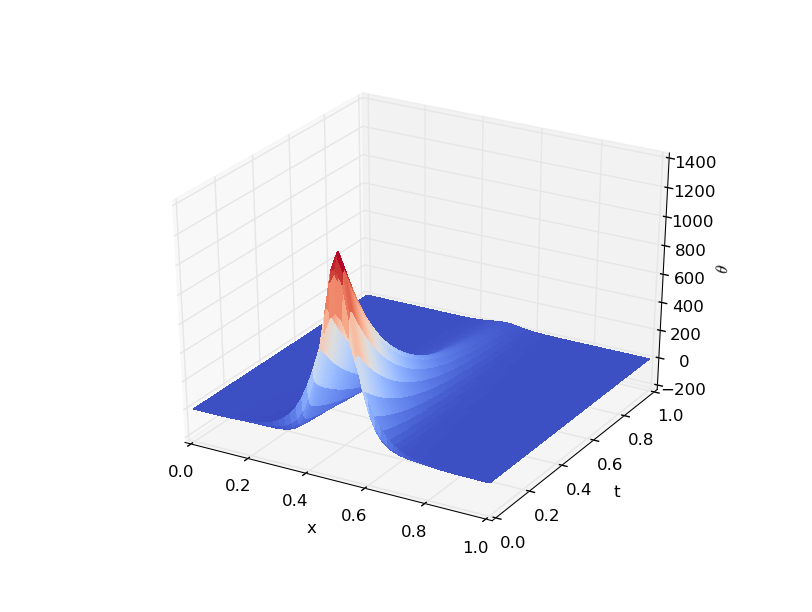
\includegraphics[width=3.5in]{re_s15}
  \caption{Управление с $\omega = (0, 0.4), \; m = 4, \; r = 30$}
  \label{fig:test2}
\end{figure}


\begin{exmp_stbur}
\end{exmp_stbur}
Пусть теперь начальное условие системы $\theta_0(x) = \frac{x^2}{G(x)}$.
Впспомним, что чем больше параметр $\tau > 0$, тем сильнее он влияет на
неустойчивость нашей системы \eqref{fluct}. Зафиксируем следующие параметры
стабилизирующего оператора управления $\omega = (0, 0.4), \ r = 30$, а параметр 
$\tau$  возмем равный $15$. Неустойчивость этой системы предемонстирована в
предыдущем параграфе (рис 2). Ниже представлен процесс стабилизации

\begin{figure}[H]
 \centering
  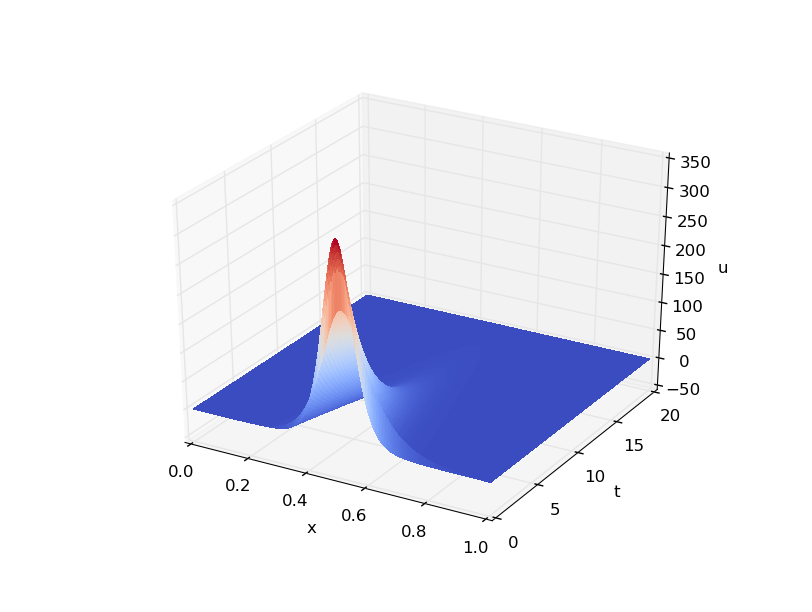
\includegraphics[width=3.5in]{re_x2_s15}
  \caption{$\omega = (0, 0.4), \; r = 30, \; m = 3$}
  \label{fig:test2}
\end{figure}

\subsubsection{Анализ параметров оператора стабилизации}

Рассмотрим ....

